\documentclass[11pt,letterpaper]{article}
\usepackage[T1]{fontenc}
\usepackage{lmodern}
\usepackage[margin=1.12in]{geometry}
\usepackage{amsmath,amssymb,amsthm,mathtools}
\usepackage{microtype}
\usepackage{tikz}
\usetikzlibrary{arrows.meta,positioning}
\usepackage{xcolor}
\definecolor{linkblue}{RGB}{30,66,107}
\usepackage[colorlinks=true,linkcolor=linkblue,citecolor=linkblue,urlcolor=linkblue]{hyperref}
\hypersetup{pdftitle={The Grothendieck homotopy hypothesis via elementary expansions},pdfauthor={OpenAI}}
\makeatletter
\newenvironment{fixedfigure}
  {\par\medskip\noindent\begin{minipage}{\linewidth}%
   \def\@captype{figure}\centering}
  {\end{minipage}\par\medskip}
\makeatother
\setlength{\emergencystretch}{1.5em}
\setlength{\parskip}{0.15em}
\numberwithin{equation}{section}
\theoremstyle{plain}
\newtheorem{theorem}{Theorem}[section]
\newtheorem{lemma}[theorem]{Lemma}
\newtheorem{proposition}[theorem]{Proposition}
\newtheorem{corollary}[theorem]{Corollary}
\theoremstyle{definition}
\newtheorem{definition}[theorem]{Definition}
\theoremstyle{remark}
\newtheorem{remark}[theorem]{Remark}
\DeclareMathOperator{\Hom}{Hom}
\DeclareMathOperator{\Mod}{Mod}
\DeclareMathOperator{\sk}{sk}
\DeclareMathOperator*{\colim}{colim}
\newcommand{\id}{\mathrm{id}}
\newcommand{\sSet}{\mathbf{sSet}}
\newcommand{\Spaces}{\mathbf{Spaces}}
\newcommand{\op}{\mathrm{op}}
\newcommand{\LL}{\mathbf L}

\title{The Grothendieck homotopy hypothesis via elementary expansions}
\author{OpenAI}
\date{September 24, 2026}
\begin{document}
\maketitle
\begin{abstract}
We prove the Grothendieck homotopy hypothesis for every Grothendieck
coherator in the Ara--Henry convention: its weak globular infinity-groupoids
recover the homotopy theory of spaces.
We also resolve Henry's pushout conjecture, showing that elementary expansions
preserve components and all homotopy groups of cellular infinity-groupoids.
\end{abstract}
\section{Introduction}\label{sec:introduction}

Grothendieck's homotopy hypothesis asks whether weak globular
infinity-groupoids describe the homotopy theory of spaces.  In
\emph{Pursuing Stacks}, the operations on paths and higher homotopies
are specified by freely adjoining coherence operations to globular
pasting diagrams \cite[Sections~9 and~12--13]{Grothendieck1983}.
A \emph{coherator} records these choices.  Maltsiniotis gave a precise
formulation in terms of coherators and their models, together with
realization and fundamental-infinity-groupoid functors
\cite{Maltsiniotis2007,Maltsiniotis2010}.
The resulting categories depend on the chosen coherator; the hypothesis
asserts that their homotopy theory recovers that of spaces.
We establish it for every coherator in the Ara--Henry convention
specified below.

The choice of algebraic model is substantive.  Simplicial sets already
model spaces through the classical realization--singular-complex
Quillen equivalence \cite[Theorem~3.6.7]{Hovey1999}.
For strict globular infinity-groupoids, however, the simply connected
homotopy types represented under a realization preserving homotopy
groups are precisely products of Eilenberg--Mac~Lane spaces \cite[Theorem~5.4]{AraStrict2013}.
The passage from strict identities to weak coherence is therefore
substantive.  Here weak equivalences are defined
inside the chosen globular algebraic category, using components and
based homotopy groups.

Henry isolated a concrete obstruction to constructing their canonical
semi-model structure \cite[Conjecture~5.3.3]{Henry2016}.  Suppose that \(X\)
is built by attaching globular cells.  Select an \(n\)-cell \(a\) of \(X\),
adjoin a new parallel \(n\)-cell \(a'\), and adjoin an \((n+1)\)-cell from
\(a\) to \(a'\).  The conjecture asserts that this free extension is a weak
equivalence.  Although the extension has an elementary retraction, its
free algebraic construction also creates composites and higher coherence
cells.  Controlling the homotopy classes of all those cells is the issue.

We use Grothendieck coherators in the convention of Ara
\cite[Sections~2.3 and~2.9--2.11]{Ara2013}, fixed by Henry in
\cite[Section~5.3]{Henry2016}; the precise definition appears in
Section~\ref{sec:preliminaries}.  Thus generating fillers of output
dimension \(j\) have pasting-scheme arity of dimension at most \(j\).
Write \(D_j\) for the free model on a \(j\)-globe and \(\partial D_j\)
for its boundary, with \(\partial D_0=\varnothing\).
A model is \emph{cellular} if it is obtained from the initial model by
a possibly transfinite sequence of boundary attachments.
Weak equivalences induce a bijection on components and isomorphisms on
all based homotopy groups.

\begin{samepage}
\begin{theorem}\label{thm:main}
Fix any Grothendieck coherator \(\mathcal C\).
Let \(X\) be a cellular \(\mathcal C\)-infinity-groupoid, let \(n\ge0\),
and let \(a:D_n\to X\) be any cell.  In the pushout square
\[
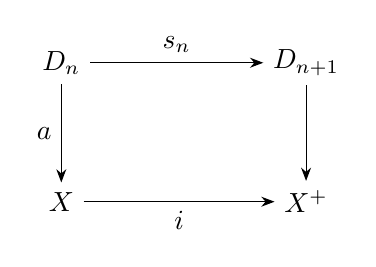
\begin{tikzpicture}[baseline=(current bounding box.center),
                   node distance=1.25cm and 2.2cm,>=Stealth]
\node (a) {\(D_n\)};
\node (b) [right=of a] {\(D_{n+1}\)};
\node (c) [below=of a] {\(X\)};
\node (d) at (b |- c) {\(X^+\)};
\draw[->] (a) -- node[above] {\(s_n\)} (b);
\draw[->] (a) -- node[left] {\(a\)} (c);
\draw[->] (b) -- (d);
\draw[->] (c) -- node[below] {\(i\)} (d);
\end{tikzpicture}
\]
where \(s_n\) is the source inclusion, the map \(i:X\to X^+\)
is a weak equivalence.
\end{theorem}
\end{samepage}

The pushout is taken in models of the fixed theory \(\mathcal C\).
The selected cell \(a\) can be any composite or coherence cell.
For \(n=0\), the extension adjoins an object and an arrow from the selected
object to it.  In particular, Theorem~\ref{thm:main} resolves Henry's
pushout conjecture affirmatively.  Henry already showed how its
finitely cellular case extends to transfinite cellular objects and their
cofibrant retracts \cite[Lemma~5.3.4]{Henry2016}; the proof here treats
arbitrary cellular objects directly.
The canonical semi-model structure and its equivalence with the homotopy
theory of spaces follow in Section~\ref{sec:consequences}.

The algebraic and homotopical sides of this question developed together.
Berger's globular theories organize operations by tree-shaped pasting
arities \cite[Definition~1.5]{Berger2002}.
Ara constructed the homotopy-group calculus and fixed-boundary tests
for weak equivalences used here \cite[Section~4]{Ara2013}.
Bourke described cellular globular theories through iterated algebraic
injectivity and proved faithfulness of their free stages
\cite[Theorems~3.12 and~5.2]{Bourke2020}.
These results make the algebraic models and their weak equivalences
precise; the remaining task is to show that elementary expansions have
the required homotopical behavior.

Henry identified the elementary pushout assertion as sufficient both
for the canonical semi-model structure and for the comparison with
spaces \cite[Theorem~5.3.5 and Corollary~5.3.13]{Henry2016}.
One route to this assertion is a functorial path construction.
Bourke's endomorphism-theory argument puts weak groupoid structures
on iterated path objects in identity type categories
\cite[Theorem~5.1]{Bourke2016}.
Within Grothendieck groupoids, Lanari constructed a globular candidate
with compositions, identities and inverses
\cite[Definitions~5.2 and~6.1, Proposition~6.2, and Theorem~6.5]{Lanari2020}.
His construction leaves the extension to compatible interpretations
of all higher operations open.  The partial paths used here are
adapted to one expansion index at a time: the already established
higher-index expansions make their representing objects contractible,
which then permits every operation of the fixed coherator to be
interpreted in its original free order.

In dimension three, Lanari obtained the canonical semi-model structure
for Grothendieck groupoids of a suitable type
\cite[Theorem~4.10]{Lanari2018}, and Henry and Lanari proved the
corresponding homotopy-hypothesis comparison \cite{HenryLanari2023}.
Their study of coskeletal and truncated globular models also supplies
context for the cutoffs used below \cite[Section~2]{HenryLanari2023}.
Taylor's later construction of algebraic coherators and Grothendieck
realizations retains a generalized pushout conjecture as a hypothesis
\cite[Conjecture~5.7 and Theorem~5.8]{Taylor2026}.
Theorem~\ref{thm:main} proves Henry's assertion for an arbitrary fixed
coherator in our convention.  Its consequence in
Section~\ref{sec:consequences} is a Quillen equivalence with spaces,
and hence independence of the resulting homotopy theory from that
choice of coherator.

\subsection*{The proof}

Section~\ref{sec:preliminaries} first expresses weak equivalence as a
lifting test with a prescribed boundary.  The proof can then work with
individual cells and their joining homotopies throughout.
The next step, in Section~\ref{sec:cutoffs-trees}, is a reflection to models in which every boundary above
dimension \(q\) has a unique filler.  It preserves all cells through \(q\).
We then hold \(q\) fixed and descend in the index \(n\) of the elementary
expansion.  The top case is immediate from the retraction and the unique
higher fillers.

At the induction step, expansions in dimensions greater than \(n\)
are already known to be weak equivalences.  A factorization argument
then gives Lemma~\ref{lem:upper-cell}: every weak equivalence built by boundary attachments
strictly above \(n\) splits and remains a weak equivalence after the
cellular pushouts needed in the proof.

The main geometric input concerns finite trees in a globular
pasting diagram.  Such a tree can be compared with a string on the same
vertices.  The composite comparison is homotopic to the identity on its
generating edges.  To pass from these individual homotopies
to a statement about all coherences, we duplicate the top generators
using only expansions already covered by the induction.
Freeness and two-out-of-three then prove contractibility of the whole
tree model (Proposition~\ref{prop:tree-contractible}).

In Section~\ref{sec:partial-cylinders}, these tree models provide partial
cylinders: an \(n\)-cell moves along an \((n+1)\)-cell, while its
lower boundary stays fixed.  Higher cylinders fit these movements
together along shared faces.  A skeletal gluing formula proves that
the objects representing such compatible tuples of cylinders are
contractible.  Interpreting the freely adjoined operations in their
chosen stage order then makes the associated path construction a functor on
models of \(\mathcal C\).  Its two endpoint maps record the ends of
each cylinder.  Individually they lift all boundary inclusions; together
they lift the current source inclusion (Proposition~\ref{prop:partial-path}).
The endpoint maps produce self-maps of the source and target that are
weak equivalences; a retract argument then proves that the expansion
itself is a weak equivalence.  Each fixed-boundary
test uses finitely many dimensions, so the end of
Section~\ref{sec:partial-cylinders} recovers
both the tested disk and its homotopy witness before the cutoff.
Section~\ref{sec:consequences} derives the canonical left semi-model
structure and applies Henry's comparison with spaces.

The main construction uses three orders: at fixed \(q\), descending
induction on the expansion index \(n\); within each step, increasing
cylinder dimension \(j\); and, for operation interpretations, the
chosen free stage order of \(\mathcal C\).
Its reusable ingredients are the reflection
preserving lower cells, the promotion of generator homotopies by
higher-dimensional expansions, and the use of partial cylinders tailored
to a single expansion index.

\section{Globular models and the weak-equivalence test}
\label{sec:preliminaries}

We first fix the algebraic conventions and prove the elementary homotopy
calculus needed below.  No model structure is used in this section.

\subsection{The fixed coherator and its free models}

A \emph{globular set} consists of sets of cells in dimensions
$0,1,\ldots$, with source and target maps satisfying the globular identities:
the source and target of a positive-dimensional cell have the same lower
source and the same lower target.  Two cells of the same dimension are
\emph{parallel} if their immediate sources and targets agree; any two
$0$-cells are parallel.  For a cell of dimension greater than $i$, write
$s_i,t_i$ for its $i$-dimensional source and target.  The representable
globular set $d_j$ is the $j$-globe, and $\partial d_j$ is its boundary;
$\partial d_0=\varnothing$.

A \emph{globular sum shape}, or \emph{pasting scheme}, is a globe or a
finite iterated amalgamation
\begin{equation}\label{eq:prelim-shape}
 S=d_{h_1}\amalg_{d_{b_1}}d_{h_2}
       \amalg_{d_{b_2}}\cdots\amalg_{d_{b_{l-1}}}d_{h_l},
 \qquad b_a<h_a,h_{a+1},
\end{equation}
where each gluing identifies a target face with a source face.  Its height
$\dim(S)$ is its largest cell dimension.  A tuple of shape $S$ in a
globular set $X$ means a globular map $S\to X$.  Let $\Theta_0$ denote the
category of these shapes and their globular maps.  Its designated sums are
the amalgamations in Equation~\eqref{eq:prelim-shape}.  The language of
globular theories and their pasting arities goes back to
Berger \cite[Definition~1.5]{Berger2002}.

\begin{definition}[The coherator convention]\label{def:coherator}
A \emph{globular theory} is a category under $\Theta_0$, with the same
objects and preserving the designated globular sums.  A
\emph{Grothendieck coherator} $\mathcal C$ is such a theory with the
following two properties.
\begin{enumerate}
\item It admits a defining tower
$\mathcal C_0=\Theta_0\to\mathcal C_1\to\cdots$ with
$\mathcal C\cong\colim_{r\ge0}\mathcal C_r$.  At stage $r+1$, one
freely adjoins a filler for each pair in a chosen set of parallel pairs
$d_{j-1}\rightrightarrows S$ in $\mathcal C_r$ satisfying
$j>0$ and $\dim(S)\le j$.  The new arrow $d_j\to S$ has that pair
as its source and target.
\item Every parallel pair $d_{j-1}\rightrightarrows S$ with
$\dim(S)\le j$ has a filler $d_j\to S$.
\end{enumerate}
Here freeness includes globular completion: the designated sums continue
to be sums after the new arrows have been adjoined.
\end{definition}

This is the admissibility convention of Ara
\cite[Sections~2.3 and 2.9--2.11]{Ara2013}, fixed in
\cite[Section~5.3]{Henry2016}.  The height bound concerns the
\emph{generating} fillers; a composite operation of output dimension $j$
can have an arity of height greater than $j$.  We retain the chosen free
cellular order throughout the proof and never replace it by an order on
output dimensions.  The tower index records the stage at which an
operation is adjoined, independently of its output dimension.  This
sequential presentation of the theory is separate from the possibly
transfinite cellular presentations of its models below.

Fix $\mathcal C$ and put $\mathcal A=\Mod(\mathcal C)$.  Its objects are
presheaves $\mathcal C^{\op}\to\mathbf{Set}$ taking the designated sums
to limits.  Equivalently, a model is a globular set with an interpretation
of each freely adjoined operation on its tuple set, subject to its two
specified face equations.  There are no additional equations equating
independently chosen fillers.  One obtains this description successively
from the universal property of each free stage: an interpretation of a
new arrow is exactly a function on tuples with the prescribed faces, and
globular completion interprets sums as tuple sets.

To make this universal-property argument explicit, let $G$ be a globular
set and let $G(S)$ be its set of tuples of shape $S$.  Form a category
$\mathcal E_G$ with objects labelled by the shapes and
\[
 \Hom_{\mathcal E_G}(S,T)=\Hom_{\mathbf{Set}}(G(T),G(S)).
\]
Composition is composition of functions in the indicated opposite
direction.  Restriction of tuples defines $\Theta_0\to\mathcal E_G$.
The designated globular sums are sums in $\mathcal E_G$: their tuple
sets are the corresponding finite limits, and maps from any fixed set
preserve those limits.  An interpretation at stage $r$ is therefore a
functor $\mathcal C_r\to\mathcal E_G$ under $\Theta_0$.  A function
interpreting a new filler, with its two prescribed faces, extends this
functor by the free-adjunction and globular-completion universal
properties \cite[Section~2.9]{Ara2013}.  Passage up the tower gives
the model.  Equations among composites follow from functoriality;
no independent filler equation is being assumed.

The forgetful functor to globular sets has a left adjoint $F$.  Set
\[
 D_j=F(d_j),\qquad \partial D_j=F(\partial d_j),\qquad
 I_j:\partial D_j\longrightarrow D_j,\qquad
 J_j:D_j\xrightarrow{s}D_{j+1}.
\]
Put $I=\{I_j\mid j\ge0\}$ and $J=\{J_j\mid j\ge0\}$.
Thus maps $D_j\to X$ are $j$-cells, and maps $\partial D_j\to X$ are
specified boundaries.  The representable presheaf $\mathcal C(-,S)$ is
a model, since the designated diagrams are sums in $\mathcal C$.
Yoneda identifies its maps into $X$ with $X(S)$, the set of tuples of
shape $S$.  Consequently
\begin{equation}\label{eq:prelim-free-shape}
 F(S)=\mathcal C(-,S),\qquad
 \Hom_{\mathcal A}(D_j,F(S))=\mathcal C(d_j,S).
\end{equation}
In particular, cells of $F(S)$ are precisely operations on the arity $S$.

An \emph{$I$-cellular extension} is a transfinite composite of pushouts
of coproducts of the $I_j$; an object is \emph{cellular} if its map from
the initial model is such an extension.  ``Finitely cellular'' means
finitely many attachments, including $I_0:\varnothing\to D_0$.\footnote{We
include the initial vertex attachment.  Although Definition~5.3.2 of
\cite{Henry2016} prints $n>0$, Section~5.3.1 specifies the empty boundary
$S_{-1}$, and Proposition~5.3.7 starts with finite globular sets and the
marked object $D_0$.  Our indexing makes that convention explicit.}
For a globular set $K$, adjoining its cells in increasing dimension is
a globular boundary-cell presentation; applying $F$ makes $F(K)$
cellular.  This does not assert that its underlying globular set has
only the cells of $K$.

The algebraic constructions below are instances of finite-limit sketch
theory; see \cite[Section~4.4, Theorems~1, 2 and~4]{BarrWells1985}.
We recall the specific finiteness facts needed here.  Models of this small
finitary essentially algebraic theory form a locally presentable
category, hence have the required limits and colimits.  Concretely,
free constructions use finite terms in the specified operations with
the prescribed matching and face equations.  Filtered colimits are
computed on the sets of cells: finite tuples and their finite matching
equations commute with filtered colimits of sets.  It follows from
adjunction that $F(K)$ is finitely presentable for every finite globular
set $K$, in particular for the disks and their boundaries.  Thus the
small-object argument of Quillen \cite{Quillen1967}, in the cellular
form of \cite[Theorem~2.1.14 and Corollary~2.1.15]{Hovey1999}, is
available for any subfamily of $I$ or $J$: adjoin cells for all lifting
problems, repeat, and take the
sequential colimit.  Each lifting problem into that colimit already
occurs at a finite stage.  These are algebraic constructions and make
no homotopical assertion.

\subsection{Homotopies, division, and change of boundary}

Contractibility of the theory supplies operations of the following
forms.  There are units $e(a):a\to a$; write $e_p^q(a)$ for their
iteration from dimension $p$ to $q$, and set $e_p^p(a)=a$.  For
$r$-cells $\alpha,\gamma$ and $i<r$ with $s_i\gamma=t_i\alpha$,
there are compositions $\gamma*_i\alpha$ and $i$-inverses
$w_i(\alpha)$.  Their exact face equations at level $i$ are
\[
 s_i(\gamma*_i\alpha)=s_i\alpha,\quad
 t_i(\gamma*_i\alpha)=t_i\gamma,\qquad
 s_iw_i(\alpha)=t_i\alpha,\quad t_iw_i(\alpha)=s_i\alpha.
\]
For $i<k<r$, their $k$-faces are obtained by applying the same
operations to the corresponding $k$-faces.  To construct them, start
in dimension $i+1$ with these prescribed faces and then proceed in
increasing dimension, prescribing the already constructed operations
on each face.  The arities are $d_r\amalg_{d_i}d_r$ and $d_r$, of
height $r$, so each required filler is admissible.  Units are fillers
of the pair consisting twice of the same operation.  Fix all these
choices once in $\mathcal C$.

Write $\alpha\sim\beta$ when there is one $(r+1)$-cell from an
$r$-cell $\alpha$ to a parallel $r$-cell $\beta$.  Units, inverses and
top-level compositions make this an equivalence relation, also for
$r=0$.  Put
\[
 \pi_0(X)=X_0/{\sim},\qquad
 \pi_r(X;u,v)=\{\alpha:u\to v\}/{\sim}\quad(r\ge1),
\]
where $u,v$ are parallel $(r-1)$-cells.  Top-level composition makes
these sets the hom sets of a groupoid on the $(r-1)$-cells having a
fixed lower boundary.  Indeed associativity, unit and inverse
expressions are parallel on the appropriate string of globes or on
a single globe; an admissible $(r+1)$-filler makes their classes equal.
Composition at any level $i$ respects homotopy: compose the given
homotopy with the unit on the fixed factor in dimension $r+1$.

The expansion argument will require a cell with an arbitrary prescribed
boundary, whereas based homotopy groups use iterated unit boundaries.
Division and change of boundary connect these two kinds of tests.
The point requiring care is that multiplication below the top level
can alter the entire boundary.  The following is the division
calculus of \cite[Lemma~4.12]{Ara2013}; we give its boundary correction
explicitly.

\begin{lemma}[Division with specified boundaries]\label{lem:prelim-division}
Fix an $r$-cell $\gamma$ and $i<r$.  Left multiplication
$\alpha\mapsto\gamma*_i\alpha$ induces a bijection from the
homotopy set at any prescribed input boundary composable with $\gamma$
to the homotopy set
at its induced output boundary.  The same holds for right
multiplication.  Empty homotopy sets are allowed.
\end{lemma}

\begin{proof}
We describe universal expressions before evaluating them in a model.
For each $k>i$, let $(g,a)$ be the generic pair of $i$-composable
$k$-cells on $d_k\amalg_{d_i}d_k$.  Initially put
\[
 U_{i+1}^k(g,a)=w_i(g)*_i(g*_i a).
\]
We inductively construct $U_h^k$ for $k\ge h>i$ with the following
two properties: its faces below $h$ equal those of $a$, and its
$l$-faces for $h\le l<k$ are $U_h^l$ evaluated on the corresponding
$l$-faces of $(g,a)$.  These statements hold for $h=i+1$ by the
exact face equations just given.  In particular $U_h^h(g,a)$ and
$a$ are parallel \emph{as operations on the generic pair of
$h$-globes}.  Choose admissible operations
\[
 c_h(g,a):a\longrightarrow U_h^h(g,a),\qquad
 d_h(g,a):U_h^h(g,a)\longrightarrow a.
\]
They have output dimension $h+1$ on an arity of height $h$.
For $k>h$, define
\begin{equation}\label{eq:prelim-normalization}
 \begin{split}
 U_{h+1}^k(g,a)={}&
 e_{h+1}^k d_h(t_hg,t_ha)\ *_h\bigl(
 U_h^k(g,a)\ *_h e_{h+1}^k c_h(s_hg,s_ha)\bigr).
 \end{split}
\end{equation}
The two compositions are defined because the old $h$-faces are
$U_h^h$ on the indicated face inputs.  Their new $h$-faces are
exactly $s_ha,t_ha$, and lower faces retain their required values.
Faces above $h$ obey the same formula in their own dimension,
by the composition and unit face equations.  This proves both
inductive properties.  Notice that parallelism for $c_h,d_h$ is
an identity in their arity, and does not result from a special
equality in the model under consideration.

Now prescribe the input boundary of an $r$-cell $\alpha$, without
assuming that such a cell exists, and let $\beta$ have the induced
boundary of $\gamma*_i\alpha$.  Begin with
$z=w_i(\gamma)*_i\beta$.  For $h=i+1,\ldots,r-1$, replace $z$ by
the right side of Equation~\eqref{eq:prelim-normalization}, with
$k=r$, $U_h^r(g,a)$ replaced by $z$, and the correction factors
evaluated at $(s_h\gamma,s_h\alpha)$ and
$(t_h\gamma,t_h\alpha)$.  These faces of $\alpha$ belong to the
\emph{prescribed boundary}.  At every stage the proper faces of
$z$ obey the universal formulas already proved, because
$\beta$ has the prescribed output boundary.  The construction
therefore finishes with an $r$-cell $K_\gamma(\beta)$ having
exactly the desired input boundary.

All correction factors depend only on $\gamma$ and that boundary.
Write $L_\gamma$ for left multiplication by $\gamma$ on homotopy classes.
Thus $K_\gamma$ is a composite of multiplication maps by fixed
cells and induces a map of homotopy sets.  On an actual input
$\beta=\gamma*_i\alpha$, it equals $U_r^r(\gamma,\alpha)$.
The latter is parallel to $\alpha$ on the generic pair of
$r$-globes, so an admissible $(r+1)$-filler shows that
$K_\gamma L_\gamma=\id$ on classes.

The same construction with left and right interchanged gives a
left inverse for every right multiplication.  Consequently all
left and right multiplication maps are injective.  Each factor
of $K_\gamma$ is one of these now-known injective maps, so
$K_\gamma$ is injective as well.  Applying this injectivity to
$K_\gamma L_\gamma K_\gamma=K_\gamma$ gives
$L_\gamma K_\gamma=\id$.  This proves bijectivity without a
nonemptiness assumption on the input set.
\end{proof}

For a vertex $x$, the group
\[
 \pi_r(X,x)=
 \pi_r\bigl(X;e_0^{r-1}(x),e_0^{r-1}(x)\bigr),\qquad r\ge1,
\]
uses top-level composition.  These are the globular homotopy groups
in Henry's statement.  A model map induces group homomorphisms,
since it preserves the chosen operations.

\begin{lemma}[Change of boundary and vertex]\label{lem:prelim-boundary-change}
The endomorphism homotopy set at any $(r-1)$-cell $u$ is naturally
in bijection with the underlying set of $\pi_r(X,x)$, where $x$
is either its source or its target vertex.  An arrow $x\to y$
gives bijections between the underlying sets of $\pi_r(X,x)$
and $\pi_r(X,y)$, natural in model maps.  If
$\pi_r(X;u,v)$ is nonempty, a chosen cell $u\to v$ gives a
bijection from the endomorphism set at $u$ to this homotopy set.
\end{lemma}

\begin{proof}
The last assertion is composition in the groupoid above.  When
$r=1$, the first assertion is the definition and change of
vertex is conjugation in the fundamental groupoid.  For $r\ge2$,
put $x=s_0u$, $a=e_0^{r-1}(x)$ and $w=u*_0a$, and abbreviate
$e(u)$ to $1_u$.  Lemma~\ref{lem:prelim-division} gives a span
of bijections
\[
 \pi_r(X;u,u)
 \xrightarrow{\ [\alpha]\mapsto[\alpha*_0 1_a]\ }
 \pi_r(X;w,w)
 \xleftarrow{\ [\beta]\mapsto[1_u*_0\beta]\ }
 \pi_r(X;a,a).
\]
For the target vertex $y=t_0u$, use
$b=e_0^{r-1}(y)$ and $w'=b*_0u$ instead: the maps are
$[\alpha]\mapsto[1_b*_0\alpha]$ and
$[\beta]\mapsto[\beta*_0 1_u]$.  Finally, for an arrow
$p:x\to y$, apply these two comparisons to
$u=e_1^{r-1}(p)$.  Naturality follows from the fixed choices of
operations; inverses of the resulting bijections are natural too.
Only set bijections are needed here.
\end{proof}

\subsection{The exact-boundary criterion}

Let $\mathcal W$ consist of the maps inducing a bijection on
$\pi_0$ and isomorphisms on all $\pi_r$ at all source vertices.
The next formulation is \cite[Theorem~4.18]{Ara2013}, with the
change-of-boundary part supplied by
\cite[Theorem~4.13 and Corollaries~4.14--4.15]{Ara2013}.

\begin{proposition}[Weak-equivalence test]\label{prop:weak-test}
For a model map $f:X\to Y$, the following are equivalent.
\begin{enumerate}
\item $f\in\mathcal W$.
\item It induces a bijection on $\pi_0$ and a bijection
\[
 \pi_r(X;u,v)\longrightarrow\pi_r(Y;fu,fv)
\]
for every $r\ge1$ and every parallel pair $u,v$ in $X$.
\item For every $r\ge0$, every specified boundary
$b:\partial D_r\to X$, and every $r$-cell $y$ of $Y$ with
boundary $fb$, there are an $r$-cell $x$ with boundary
\emph{exactly} $b$ and an $(r+1)$-cell $fx\to y$ in $Y$.
\end{enumerate}
In particular, a weak equivalence reflects homotopy between
parallel cells, including equality of components for vertices.
\end{proposition}

\begin{proof}
Suppose (1) holds.  Lemma~\ref{lem:prelim-boundary-change} shows
that $f$ is bijective on every endomorphism homotopy set.
We prove (2) by induction on $r$.  First address existence of
a class: if a $1$-cell joins $fu$ to $fv$, injectivity on
$\pi_0$ gives a cell $u\to v$.  If $r>1$ and a target
$r$-cell joins $fu$ to $fv$, then $fu,fv$ represent the same
class in the appropriate $(r-1)$-dimensional homotopy set.
Injectivity already proved in dimension $r-1$ gives a source
$r$-cell $u\to v$.  Thus a nonempty target homotopy set has
a nonempty source homotopy set.  Choose a source joining cell;
composition with it and its image identifies the map on these
homotopy sets with the map on endomorphism sets.  The latter
is bijective.  If the target set is empty, the source is empty
as well, so the assertion also holds in that case.

Condition (2) immediately gives (3), using surjectivity on
$\pi_0$ when $r=0$.  Conversely (3) gives surjectivity on
$\pi_0$ and on every homotopy set at a source boundary.
If parallel source $r$-cells have homotopic images, apply
(3) in dimension $r+1$ to their exact boundary and the target
joining cell.  This produces a source joining cell.  For
$r=0$ it proves injectivity on $\pi_0$, and for $r\ge1$
it proves injectivity on the indicated homotopy sets.  Hence
(2) follows, and its based instances give (1).
\end{proof}

\begin{lemma}[Closure properties]\label{lem:weak-closure}
The class $\mathcal W$ has two-out-of-three, is closed under
retracts, and is closed under filtered colimits of arrows.
Consequently a transfinite composite of weak equivalences is
a weak equivalence.
\end{lemma}

\begin{proof}
For two-out-of-three, use the induced maps of components and
based groups.  In the case where $f$ and $gf$ are weak
equivalences, a vertex of the intermediate model is joined to
some $f(x)$, by surjectivity of $\pi_0(f)$.
Lemma~\ref{lem:prelim-boundary-change} transfers bijectivity
of the homomorphism induced by $g$ at $f(x)$ to that vertex.
The other two cases follow directly by cancellation of
bijections.  Retract closure follows from
Proposition~\ref{prop:weak-test}(3), even for a retract of
underlying globular arrows: apply its disk and homotopy
witnesses in the larger arrow and retract them.

For a filtered colimit of weak equivalences, the prescribed
boundary, target disk, and their finitely many matching
equations in Proposition~\ref{prop:weak-test}(3) all occur
together at some stage.  Apply the test there and map its
two witnesses to the colimit.  Finally, transfinite induction
handles a transfinite composite: use composition at successor
stages and, at a limit, apply filtered-colimit closure to the
arrows from the constant initial stage to the preceding stages.
No injectivity of the transition maps is required.
\end{proof}

\begin{definition}\label{def:prelim-contractible}
A model $X$ is \emph{contractible} if $X\to1$ belongs to
$\mathcal W$.  Equivalently, $X$ is nonempty and every
parallel pair of cells has a joining cell.
\end{definition}

The equivalence in this definition is
Proposition~\ref{prop:weak-test}(3) applied to $X\to1$:
the condition in dimension zero is nonemptiness, and in
positive dimension it is exact boundary filling.  Equivalently,
$X\to1$ lifts against every $I_j$.  Thus a map from any
cellular domain extends across an $I$-cellular extension
whenever its target is contractible.

For a set of maps $K$, write $K\text{-}\mathrm{inj}$ for the maps
with the right lifting property against every member of $K$.

\begin{lemma}[Lifting tests]\label{lem:lifting-test}
If $f\in\mathcal W$ has the right lifting property against
$J_j$, it has the right lifting property against $I_j$.
Moreover
\[
 I\text{-}\mathrm{inj}
   =\mathcal W\cap J\text{-}\mathrm{inj}.
\]
Every model maps to the terminal model with the right lifting
property against all $J_j$.
\end{lemma}

\begin{proof}
For a square against $I_j$, Proposition~\ref{prop:weak-test}
provides an approximate $j$-cell lift $x$ and a target
$(j+1)$-cell $H:fx\to y$.  Lifting $H$ against
$J_j:D_j\to D_{j+1}$ with prescribed source $x$ gives a
$(j+1)$-cell whose target is a strict lift of $y$ with the
specified boundary.  This also proves the assertion for
$j=0$.

An $I$-injective map satisfies the test strictly, using the
unit on the target disk as its homotopy, so it belongs to
$\mathcal W$.  Each $J_j$ is the composite of two boundary
attachments: first adjoin the parallel target $j$-cell using
$I_j$, then the joining $(j+1)$-cell using $I_{j+1}$.
Thus $I$-injectivity implies $J$-injectivity, and the first
paragraph proves the reverse inclusion in the displayed
equality.  Finally a $J_j$-lifting problem for $X\to1$
is solved by the unit on its prescribed source cell.
\end{proof}

The same unit defines a retraction $D_{j+1}\to D_j$ of
$J_j$.  Its pushout along any specified cell therefore has
a retraction as well.  A transfinite composite of such
pushouts has compatible retractions to its initial object:
choose the retraction at each successor and use the induced
map out of the colimit at each limit.  The existence of these
retractions alone does not establish weak equivalence.

\section{Coskeletal cutoffs and contractible trees}
\label{sec:cutoffs-trees}

We first establish two facts without using any elementary-expansion
assertion: higher cell attachments preserve lower cells, and free models
on globular sums are contractible.  We then fix a finite cutoff and set
up a descending induction.  Within one step of that induction, the
already established higher-dimensional expansions will suffice to
contract the tree diagrams needed for partial cylinders.

\subsection{The cutoff reflector}

Coskeletal globular models and their relation to truncated models are
studied in \cite[Section~2]{HenryLanari2023}.  We construct the reflector
needed here directly, keeping the chosen free order of the coherator.

For an integer $q\geq0$, call a model \emph{$q$-coskeletal} if every
globular boundary of dimension $j>q$ has exactly one filler.  Thus the
restriction map
\[
 \Hom(D_j,Y)\longrightarrow\Hom(\partial D_j,Y)
\]
is bijective for every $j>q$.  Let $\mathcal A_q$ be the full subcategory
of such models.  The uniqueness begins in dimension $q+1$; distinct
parallel $q$-cells are retained.
To recover a homotopy-class test in dimension $k$, we will choose
$q\geq k+1$, retaining both the tested cells and their joining homotopies.

\begin{lemma}[Cutoff reflector]\label{lem:cutoff}
The inclusion $\mathcal A_q\subseteq\mathcal A$ has a left adjoint
$R_q$.  Its unit $X\longrightarrow R_qX$ is bijective on the sets of
cells in every dimension at most $q$.  For $0\leq k<q$, the same
construction gives the reflector $\mathcal A_q\to\mathcal A_k$,
and $R_kR_q$ is naturally isomorphic to $R_k$.
\end{lemma}

\begin{proof}
On underlying globular sets, retain the cells and face maps of $X$
through dimension $q$.  In successive dimensions $j>q$, put one
$j$-cell over each parallel pair of $(j-1)$-cells.  Denote the resulting
globular set by $Z$.  There is a canonical globular map $\eta:X\to Z$,
equal to the identity through $q$.

To interpret the theory on $Z$, follow the \emph{given free cellular
presentation of $\mathcal C$ in its original order}.  Maintain that
$\eta$ respects the part of the theory already interpreted.  Suppose
a newly adjoined generating operation has output dimension $j$ and
arity $S$.  Its two prescribed faces are operations of the earlier
theory.

If $j\leq q$, the generating arity bound
$\dim(S)\leq j$ in Definition~\ref{def:coherator} makes the tuple sets
on $S$ in $X$ and $Z$ identical.  Use the original interpretation in
$X$.  Its prescribed face equations hold in $Z$: the tuple comes
from $X$, and $\eta$ already respects both earlier face operations.
It also respects the new operation, since it is the identity in
dimension $j$.

If $j>q$, the earlier interpretation gives a parallel boundary in
$Z$, and the new operation is its unique filler.  The image under
$\eta$ of the operation in $X$ has that boundary, so uniqueness again
shows compatibility with $\eta$.  At a limit stage take the union of
the preceding interpretations.  Freeness of the presentation now
gives a model structure on $Z$.  This argument places no bound on
the arities of \emph{composite} face operations and does not reorder
generators by dimension.

For a $q$-coskeletal model $Y$, a model map $f:X\to Y$ has a unique
globular factorization through $\eta$: use $f$ through dimension $q$
and unique fillers thereafter.  This factorization is a model map.
For a generator of output at most $q$, every tuple comes from $X$;
for a higher generator, preservation follows from uniqueness in
$Y$.  This proves the adjunction.  Starting with $X\in\mathcal A_q$
and performing the construction at $k<q$ proves the remaining
statements by the same universal property.
\end{proof}

Write $F_q=R_qF$ for the free $q$-coskeletal model functor.  Since
$R_q$ is a left adjoint, it preserves actual algebraic pushouts and
cellular presentations.  In $\mathcal A_q$ the images of $I_j$ and
$J_j$ are isomorphisms for $j>q$.  The image of $J_q$ freely adjoins
a parallel $q$-cell; its joining $(q+1)$-cell is forced by uniqueness.
This description includes all operations of the fixed theory on the
new cell.

Filtered colimits of $q$-coskeletal models, computed in
$\mathcal A$, remain $q$-coskeletal: both disks and their finite
boundaries commute with such colimits, so the required restriction
maps remain bijective.  Consequently filtered colimits in
$\mathcal A_q$ are computed on cells as well.  The adjunction for
$F_q$ now shows that $F_q(K)$ is finitely presentable whenever $K$
is a finite globular set.  The category $\mathcal A_q$ is
cocomplete by reflection, and the same ordinary small-object
construction is therefore available for its disk and boundary
maps.  No model structure is being used.

\begin{lemma}[Higher attachments preserve lower cells]
\label{lem:high-cells}
Fix $k\geq0$.  In $\mathcal A$, any relative cellular extension using
only $I_j$ with $j>k$ is bijective on all cells through dimension $k$.
The same holds in $\mathcal A_q$ whenever $k<q$.  Consequently these
conclusions also hold for relative extensions using only $J_j$
with $j>k$.
\end{lemma}

\begin{proof}
The reflection of $I_j$ into $\mathcal A_k$ is an isomorphism when
$j>k$: every $k$-coskeletal model has a unique filler of every
$j$-boundary.  Reflect a pushout, a coproduct of attachments, or a
transfinite composite of such maps.  Colimit preservation makes its
reflection an isomorphism.  Since both reflection units preserve
the cells through $k$, the original map is bijective on those cells.
Within $\mathcal A_q$, use the further reflection to $\mathcal A_k$.
Finally, $J_j$ is the composite of an $I_j$ attachment, adjoining its
new target $j$-cell, and an $I_{j+1}$ attachment, adjoining the
comparison cell.
\end{proof}

\subsection{Spines of globular sums}

We use an explicit recursive description of finite globular-sum
shapes.  For nonempty shapes $S_1,\ldots,S_p$, write
$[S_1,\ldots,S_p]$ for the shape with vertices
$v_0,\ldots,v_p$ whose cells over each consecutive pair
$(v_{i-1},v_i)$ form the suspension of $S_i$.  Suspension raises
dimensions by one and gives the suspended shape these two vertices
as poles.  Every shape is either a vertex or has this form.  To see
this from a table of dimensions, split its ordered amalgamation at
all gluings in dimension zero and lower every dimension in each
remaining block by one.  Repeating gives the stated recursion.

For a shape $S$, let $v(S)$ denote its first vertex.  Define a
subshape $T_m(S)$, for $m\geq0$, recursively.  A vertex is fixed, and
for $S=[S_1,\ldots,S_p]$ put
\begin{equation}\label{eq:spine-recursion}
\begin{split}
 T_0(S)&=[v(S_1),\ldots,v(S_p)],\\
 T_m(S)&=[T_{m-1}(S_1),\ldots,T_{m-1}(S_p)]\qquad(m\geq1).
\end{split}
\end{equation}
In the first line each $v(S_i)$ denotes the one-vertex subshape of
$S_i$.  Thus at depth $m$ the construction keeps every vertex and
one generating edge between consecutive vertices.  A branch ending
before that depth is retained in full.

\begin{lemma}[Finite spine]\label{lem:spine}
For every finite globular-sum shape $S$ and every $m\geq0$, the
subshape $T_m(S)$ has height at most $m+1$ and contains every cell of
$S$ through dimension $m$.  The inclusion $T_m(S)\to S$ is a finite
composite of pushouts of the globular source inclusions
$d_j\to d_{j+1}$ with $j>m$.
\end{lemma}

\begin{proof}
First, every shape $S$ can be built from $v(S)$ by finitely many
source inclusions $d_j\to d_{j+1}$ with $j\geq0$.  This is induction
on the recursive description.  If $S$ is a vertex there is nothing
to attach.  Otherwise, for $S=[S_1,\ldots,S_p]$, first build the
outer vertex string by source inclusions in dimension zero, using
in its $i$th slot the edge corresponding to $v(S_i)$.  Then build
each $S_i$ from $v(S_i)$ by the induction hypothesis and suspend its
attachments into that slot.  Under this suspension an elementary
pair of dimensions $(j,j+1)$ becomes one of dimensions $(j+1,j+2)$,
with exactly the same source-attachment description.  This follows
directly from the face maps: the two added cells acquire the fixed
outer poles, and their other faces are the suspended old faces.

The height and lower-cell claims for $T_m$ now follow directly from
Equation~\eqref{eq:spine-recursion}.  For the attachment claim when
$m=0$, rebuild each $S_i$ from $v(S_i)$ as above.  All these
attachments are suspended once, so their indices are at least
one.  For $m\geq1$, the induction hypothesis for
$T_{m-1}(S_i)\to S_i$ uses indices $j>m-1$; suspending gives indices
$j+1>m$.  Apply this construction in every slot.  There are finitely
many slots and attachments because $S$ is finite.
\end{proof}

Contractibility of free globular sums is established in
\cite[Proposition~3.8]{Lanari2020}.  The spine argument below proves
the statement directly in our convention and also gives its reflected form.

\begin{proposition}[Contractibility of free shapes]
\label{prop:shape-contractible}
For every nonempty finite globular-sum shape $S$, the models $F(S)$
and $F_q(S)$ are contractible, for every $q\geq0$.
\end{proposition}

\begin{proof}
Let $a,b$ be parallel $m$-cells of $F(S)$, where $m\geq0$ and in
dimension zero there is no parallelism condition.  By
Lemmas~\ref{lem:spine} and~\ref{lem:high-cells}, the map
$F(T_m(S))\to F(S)$ is bijective on every cell set through $m$.
Hence $a,b$ have unique lifts $a',b'$ there, and the lifts are
parallel: their lower faces agree by the same injectivity.

The free model on a globular-sum shape is represented by that
object of $\mathcal C$.  Thus $a',b'$ are a parallel pair of theory
arrows with domain the $m$-globe and codomain $T_m(S)$.
Since $\dim(T_m(S))\leq m+1$, this pair is admissible for a filler
of dimension $m+1$.  Contractibility of $\mathcal C$ supplies such a
filler.  Its image joins $a$ to $b$ in $F(S)$.
The model is nonempty because $S$ has a vertex, so the
contractibility criterion of Proposition~\ref{prop:weak-test}
applies.  No assertion about weak equivalences of elementary
attachments was used here.

For $F_q(S)$, a parallel pair of $m$-cells with $m<q$ lifts to
$F(S)$ by Lemma~\ref{lem:cutoff}; the filler just constructed is
preserved through dimension $m+1\leq q$.  If $m\geq q$, the
required filler has dimension $m+1>q$ and exists uniquely.  The
vertex is retained, so $F_q(S)$ is also contractible.
\end{proof}

\subsection{The descending induction and its upper-cell consequence}

Fix $q\geq0$.  Until the cutoff is removed in the next section,
all constructions take place in $\mathcal A_q$.  We keep the notation
$F_q$ for free models, and write $D_j,\partial D_j,I_j,J_j$ for
their images under $R_q$.  Weak equivalence means the same
component and based-homotopy-group test on these models; all the
properties in Section~\ref{sec:preliminaries} remain applicable.

For $0\leq n\leq q$, let $\mathsf E(q,n)$ be the following assertion:
\begin{quote}
For every cellular object $X\in\mathcal A_q$ and every model map
$a:D_n\to X$, the actual pushout of $J_n$ along $a$ is a weak
equivalence.
\end{quote}
Here cellular objects and extensions may have any set-sized
transfinite presentation.  The attaching map $a$ need not select
a presentation generator.  We will prove $\mathsf E(q,n)$ by
descending induction on $n$.

\begin{lemma}[Top-dimensional base case]\label{lem:cutoff-base}
The assertion $\mathsf E(q,q)$ holds for every $q\geq0$.
\end{lemma}

\begin{proof}
Let $i:X\to Y$ be a pushout of $J_q$.  It has a retraction
$r:Y\to X$, obtained by sending the new $q$-cell to the attaching
cell and its comparison to a unit.  For $q>0$,
Lemma~\ref{lem:high-cells} shows that $i$ is bijective on cells
through dimension $q-1$.

Check the exact-boundary criterion of
Proposition~\ref{prop:weak-test} in dimension $d$.  If $d<q$, the
given $d$-cell of $Y$ comes from a unique $d$-cell of $X$, whose
boundary is the prescribed one by injectivity on lower cells.
Its image is the given cell, so its unit supplies the homotopy.
If $d=q$, apply $r$ to the given cell.  Its boundary is the
prescribed boundary because $ri=\id_X$, and its image is parallel
to the given cell.  These two $q$-cells have a unique joining
$(q+1)$-cell.  If $d>q$, the prescribed source boundary has a
unique filler in $X$, whose image is the given filler in $Y$.
This proves the criterion in every dimension.
For $q=0$, the first case is absent; the same retraction and
unique-arrow argument proves the dimension-zero case directly.
\end{proof}

For the rest of this section and the construction in the next,
fix $0\leq n<q$ and assume $\mathsf E(q,j)$ for every
$n<j\leq q$.  Call an index \emph{upper} if it is strictly greater
than $n$.  Thus an upper $I$-cellular extension uses only $I_j$
with $j>n$, and likewise for upper $J$-cellular extensions.
Every upper $J$-cellular extension with cellular source is in
$\mathcal W$: the successor stages use the induction hypothesis
(or an isomorphism for $j>q$), and limit stages use
Lemma~\ref{lem:weak-closure}.  Every intermediate object remains
cellular, since each $J_j$ is a composite of two boundary
attachments.

\begin{lemma}[Upper-cell splitting and pushout]
\label{lem:upper-cell}
Suppose $i:U\to V$ is an upper $I$-cellular extension, $U$ is
cellular, and $i\in\mathcal W$.  Then $i$ admits a retraction.
For every map $U\to U'$ with $U'$ cellular, the pushout
\[
 U'\longrightarrow U'\amalg_U V
\]
also belongs to $\mathcal W$.
\end{lemma}

\begin{proof}
Apply the ordinary small-object construction with the upper
$J_j$ to factor $i$ as
\[
 U\xrightarrow{\,a\,}Z\xrightarrow{\,p\,}V,
\]
where $a$ is upper $J$-cellular and $p$ lifts against every upper
$J_j$.  The preceding induction hypotheses imply $a\in\mathcal W$,
so $p\in\mathcal W$ by two-out-of-three.  By
Lemma~\ref{lem:lifting-test}, $p$ lifts against every upper $I_j$:
the approximate lift of a $j$-cell is corrected by lifting its
$(j+1)$-dimensional homotopy against $J_j$.  In particular the
lowest index required is $J_{n+1}$, which is already available.

Since $i$ is upper $I$-cellular, there is a map $s:V\to Z$ with
$si=a$ and $ps=\id_V$.  Thus, in the category under $U$, the map
$i$ is a retract of $a$.
Each individual $J_j$ attachment admits a unit retraction.  A
transfinite composite of such attachments also retracts to its
initial object: choose the maps back recursively at successor
stages, and use their compatible colimit map at a limit stage.
Let $t:Z\to U$ be the resulting retraction of $a$.  Then $ts$ is
a retraction of $i$.

Push the retract diagram out along $U\to U'$.  The pushout of
$i$ is a retract of the pushout of $a$, and the latter is upper
$J$-cellular with cellular source $U'$.  It is therefore in
$\mathcal W$ by the induction hypotheses.  Retract closure proves
the claim.
\end{proof}

\subsection{Trees in a fixed globular dimension}

Define a \emph{tree diagram at depth $n$} as follows.  At depth zero,
it is a finite nonempty oriented tree, regarded as a globular set
of dimensions zero and one; a single vertex is allowed.  At
depth $n>0$, it is either a vertex or a string
$[K_1,\ldots,K_p]$ with every $K_i$ a tree diagram at depth $n-1$.
Such a diagram $K$ is a finite globular set of height at most
$n+1$.  In each depth-$n$ slot, the tree vertices are $n$-cells
with one common lower boundary, and its edges are $(n+1)$-cells.
All orientations of the edges are allowed.  At $n=0$ the lower
boundary condition is empty.

The free model $F_q(K)$ is cellular: attach its finitely many
globular cells along their boundaries in increasing dimension and
apply the free functor.  Its finite generating globular set must
be distinguished from the generally infinite collection of cells
created by the operations of $\mathcal C$.

\begin{fixedfigure}
\centering
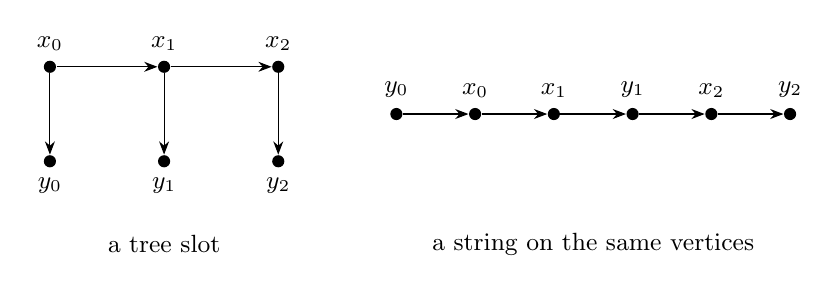
\begin{tikzpicture}[>=Stealth,
    vertex/.style={circle,fill=black,inner sep=1.55pt},
    every node/.style={font=\small}]
\begin{scope}
\node[vertex,label=above:\(x_0\)] (x0) at (0,1.2) {};
\node[vertex,label=above:\(x_1\)] (x1) at (1.45,1.2) {};
\node[vertex,label=above:\(x_2\)] (x2) at (2.9,1.2) {};
\node[vertex,label=below:\(y_0\)] (y0) at (0,0) {};
\node[vertex,label=below:\(y_1\)] (y1) at (1.45,0) {};
\node[vertex,label=below:\(y_2\)] (y2) at (2.9,0) {};
\draw[->] (x0) -- (x1);
\draw[->] (x1) -- (x2);
\draw[->] (x0) -- (y0);
\draw[->] (x1) -- (y1);
\draw[->] (x2) -- (y2);
\node at (1.45,-1.05) {a tree slot};
\end{scope}
\begin{scope}[xshift=4.4cm]
\node[vertex,label=above:\(y_0\)] (z0) at (0,0.6) {};
\node[vertex,label=above:\(x_0\)] (z1) at (1,0.6) {};
\node[vertex,label=above:\(x_1\)] (z2) at (2,0.6) {};
\node[vertex,label=above:\(y_1\)] (z3) at (3,0.6) {};
\node[vertex,label=above:\(x_2\)] (z4) at (4,0.6) {};
\node[vertex,label=above:\(y_2\)] (z5) at (5,0.6) {};
\draw[->] (z0) -- (z1);
\draw[->] (z1) -- (z2);
\draw[->] (z2) -- (z3);
\draw[->] (z3) -- (z4);
\draw[->] (z4) -- (z5);
\node at (2.5,-1.05) {a string on the same vertices};
\end{scope}
\end{tikzpicture}
\caption{A tree in one depth-\(n\) slot and a string on the same vertices.
Vertices are \(n\)-cells and arrows are
\((n+1)\)-cells.  The comparison maps between the free models fix the
named vertices and send generating edges to composites along connecting
paths, using inverses where necessary.  The \(J_{n+1}\)-duplication
argument in Proposition~\ref{prop:tree-contractible} promotes the
resulting edge homotopies to a statement about the full models.}
\label{fig:tree-string}
\end{fixedfigure}


\begin{proposition}[Contractibility of tree diagrams]
\label{prop:tree-contractible}
Under the fixed-cutoff induction hypotheses above, $F_q(K)$ is
contractible for every tree diagram $K$ at depth $n$.
\end{proposition}

\begin{proof}
In each depth-$n$ slot, order its tree vertices in any way and
replace the tree by the forward linear string on those same
labeled vertices.  A singleton remains a singleton.  The resulting
globular set $K^{\mathrm{lin}}$ is a globular-sum shape, and its
cells through dimension $n$ are canonically the same as those of
$K$; Figure~\ref{fig:tree-string} illustrates one slot.  Reordering
within a slot leaves unchanged any outer poles and
every earlier concatenation or suspension.  Put
\[
 A=F_q(K),\qquad L=F_q(K^{\mathrm{lin}}).
\]
The model $L$ is contractible by
Proposition~\ref{prop:shape-contractible}.

There are model maps
\[
 f:A\longrightarrow L,\qquad g:L\longrightarrow A
\]
fixing the generating cells through dimension $n$.  To define
$f$, send each tree edge to a composite along the path between
its endpoints in the corresponding line, using inversion for
any backward traversal.  Define $g$ using paths in the tree.
All compositions are at level $n$.  Within one slot the vertices
are parallel $n$-cells, so these assignments have exactly the
required faces.  They extend to model maps by the free universal
property.

For each $(n+1)$-dimensional generating edge $e$ of $K$, choose
a cell
\begin{equation}\label{eq:tree-generator-homotopy}
 \alpha_e:e\longrightarrow gf(e)
 \qquad\text{of dimension }n+2\text{ in }A.
\end{equation}
Such a cell exists by the groupoid calculus of
Section~\ref{sec:preliminaries}.  Indeed, $gf(e)$ represents a
walk in the original tree with the same endpoints as $e$.
Here an inverse of a composite is expanded at the level of homotopy
classes, using uniqueness of inverses in the hom-set groupoid.
Successively delete backtracking pairs from this walk.  A walk
in a tree without backtracking is the unique simple path between
its endpoints, here the edge $e$.  Associativity, units, and
inverse cancellation hold for $(n+1)$-cells modulo
$(n+2)$-cell homotopy, so the two cells represent the same class.
The homotopy relation is given by existence of a single joining
cell, giving Equation~\eqref{eq:tree-generator-homotopy}.

We next turn these homotopies on generators into a statement
about the whole model.  For every such edge $e$, adjoin a
duplicate $e'$ with the same boundary and a cell
$\delta_e:e\to e'$ of dimension $n+2$.  Let $Q$ be the resulting
model and $a_0:A\to Q$ its canonical map.  These are finitely
many $J_{n+1}$ attachments, so $a_0\in\mathcal W$ by the already
proved higher-index case.  Define a second model map
$a_1:A\to Q$ by fixing every generator through dimension $n$
and sending $e$ to $e'$.  This is permitted because
$A=F_q(K)$ and $K$ has no generators above dimension $n+1$.
The face equations of this globular assignment are the only
conditions needed to extend it to the full model.

There is a common retraction $r:Q\to A$: keep the original
generators, send $e'$ to $e$, and send $\delta_e$ to a unit on
$e$.  Thus $ra_0=ra_1=\id_A$.  Two-out-of-three gives first
$r\in\mathcal W$ and then $a_1\in\mathcal W$.
Likewise Equation~\eqref{eq:tree-generator-homotopy} defines a
model map $h:Q\to A$ which is the identity on the original copy,
sends $e'$ to $gf(e)$, and sends $\delta_e$ to $\alpha_e$.
The free universal property gives
\[
 ha_0=\id_A,\qquad ha_1=gf.
\]
It follows that $h\in\mathcal W$ and $gf\in\mathcal W$.
This promotion uses only $J_{n+1}$, not $J_n$.

The map $gf$ factors through the contractible model $L$.  Hence
its map on components factors through a singleton and its maps
on positive based homotopy groups factor through trivial groups.
Since these maps are respectively bijective and isomorphisms,
$A$ has one component and trivial homotopy groups.  It is
nonempty, so it is contractible.

When $q=n+1$, the attachments used above are precisely $J_q$,
whose case was proved in Lemma~\ref{lem:cutoff-base}.  They retain
the duplicate $q$-generators, while the joining $(q+1)$-cells
are unique.  The definitions of $a_1,r,h$ still have exactly
their stated universal properties.  Thus this boundary case
requires no additional induction step.
\end{proof}

\subsection{Whiskers on globular sums}

Let $S$ be a finite globular-sum shape with $\dim(S)\leq q$.
For $\epsilon\in\{0,1\}$, define $H_\epsilon(S)$ by starting
with $F_q(S)$ and, for each actual $n$-cell $x$ of the globular
set $S$, adjoining a duplicate $x'$ with the same boundary and
one $(n+1)$-cell joining them.  Orient the join $x\to x'$ when
$\epsilon=0$ and $x'\to x$ when $\epsilon=1$.  Every original
higher generating cell of $S$ keeps its original boundary.
These are cellular constructions: attach each duplicate along
its boundary, then its joining cell.  For $n=0$ the duplicate
attachment is an attachment of a vertex.  If $S$ has no
$n$-cells, set $H_\epsilon(S)=F_q(S)$.

\begin{proposition}[Contractibility after adjoining whiskers]
\label{prop:whiskered-shape}
Under the fixed-cutoff induction hypotheses above,
$H_\epsilon(S)$ is contractible for both choices of $\epsilon$.
The same conclusion holds if the orientation of the join is
chosen independently for each $n$-cell of $S$.
\end{proposition}

\begin{proof}
Set $S'=T_n(S)$.  It contains exactly the same $n$-cells as $S$,
so the same duplicates and joins can be adjoined to either
shape.  In $S'$ every slot at depth $n$ is a linear string or a
singleton.  Adding one leaf and its edge at each vertex turns
each such slot into a finite oriented tree.  Thus
$H_\epsilon(S')$ is the free model on a tree diagram at depth
$n$, and is contractible by
Proposition~\ref{prop:tree-contractible}.  The same argument
allows independent orientations.

By Lemma~\ref{lem:spine}, $S'\to S$ is a finite composite of
source attachments with indices strictly greater than $n$.
Those attachments add no further $n$-cells.  Perform them after
adjoining the fixed set of duplicates and joins.  Their original
attaching maps use the retained generators of $S$ and their
original faces, so the resulting model is exactly
$H_\epsilon(S)$ by the pushout universal properties.  Therefore
$H_\epsilon(S')\to H_\epsilon(S)$ is upper $J$-cellular.  Its
source and all intermediate objects are cellular, so the
descending induction hypotheses make it a weak equivalence.
Contractibility follows from that of $H_\epsilon(S')$.
If the recursion ends before depth $n$, there are no joins in
that branch and it remains unchanged throughout.
\end{proof}

The hypotheses $0\leq n<q$ and $\mathsf E(q,j)$ for $j>n$
remain in force in the next section.  The tree and whisker
propositions have established the needed non-pasting diagrams
using only those hypotheses; the assertion $\mathsf E(q,n)$
itself is still to be proved.

\section{Partial cylinders and elementary expansions}
\label{sec:partial-cylinders}

Continue to work at a fixed cutoff \(q\).  Fix \(0\le n<q\), and
assume the descending induction hypothesis for every index greater than
\(n\), with arbitrary cellular starting objects.  In this section,
write \(F\) for \(F_q\), and retain \(D_j,\partial D_j,I_j,J_j\)
for their images in \(\mathcal A_q\); an \emph{upper} attachment has index greater than
\(n\).  In particular, Lemma~\ref{lem:upper-cell} and
Propositions~\ref{prop:tree-contractible} and
\ref{prop:whiskered-shape} are available.

Our goal is a functor \(\mathcal P\) with natural endpoint maps
\(p_0,p_1:\mathcal P Y\to Y\).  Each endpoint must lift every
boundary inclusion, while the pair \((p_0,p_1)\) must lift \(J_n\).
Here is how these properties will prove the induction step.  For a
cellular \(X\), the individual lifting property supplies a section
\(h:X\to\mathcal P X\) of \(p_0\), and \(u=p_1h\) is a weak
equivalence.  For an elementary expansion \(i:X\to Y\) with its
unit retraction \(r:Y\to X\), the joint lifting property extends
this comparison over \(Y\) and makes \(iur\) a weak equivalence.
The map \(iu\) is then a retract of \(iur\), so retract closure
and two-out-of-three will give the desired weak equivalence \(i\).
We construct the representing cylinder objects first, then interpret
the operations of \(\mathcal C\) to obtain this functor and its
endpoint properties.

\subsection{The cylinder objects}

Representing path cells by maps out of a coglobular cylinder follows
the strategy of Lanari
\cite[Definitions~5.2--5.3 and~6.1]{Lanari2020}.
Here the cylinders depend on the fixed cutoff and expansion index;
their upper completions will support the descending induction and
the interpretation of every operation of the chosen coherator.

The object \(P_j\) will represent a cylinder on a \(j\)-cell:
a map \(P_j\to Y\) specifies that cylinder in \(Y\), with two
endpoint \(j\)-cells.  The endpoints coincide below dimension \(n\).
In dimension \(n\), a cylinder is a single \((n+1)\)-cell joining
them.  In higher dimensions we will attach cells to make these data
compatible along their common faces.

We construct a coglobular diagram \(P_0,\ldots,P_q\), together with
two maps of coglobular diagrams
\[
             e_\epsilon:D_\bullet\longrightarrow P_\bullet,
             \qquad \epsilon=0,1.
\]
For a globular set \(S\) of dimension at most \(q\), put
\begin{equation}\label{eq:cylinder-realization}
 P(S)=\colim_{(d_j\longrightarrow S)}P_j.
\end{equation}
The indexing category is the category of cells and their faces in
\(S\).  In particular, the structure maps into \(P_j\) specify a
map \(P(\partial d_j)\to P_j\), and the endpoint maps induce
\(e_\epsilon(S):F(S)\to P(S)\).  This notation will also be used
while only the cylinder objects needed by \(S\) have been constructed.

Given the objects in dimensions below \(j\), a boundary cylinder and
one prescribed endpoint are represented by \(A_j^\epsilon\); prescribing
both endpoints instead gives \(A_j^{01}\).  Their precise definitions are
\begin{align}
 A_j^\epsilon
   &=P(\partial d_j)\amalg_{\partial D_j,e_\epsilon}D_j,
       \label{eq:cylinder-one-sided}\\
 A_j^{01}
   &=P(\partial d_j)
       \amalg_{\partial D_j\amalg\partial D_j}
                    (D_j\amalg D_j).
       \label{eq:cylinder-two-sided}
\end{align}
In Equation~\eqref{eq:cylinder-two-sided}, the first attaching map uses
both endpoints on the boundary, and the second uses the two boundary
inclusions.  Empty boundaries have their usual meaning at \(j=0\).

The two domains have different tasks.  The two-sided domain records
the boundary and both endpoint values that an operation on cylinders
must preserve.  We will choose \(P_j\) receiving these data.  The
resulting one-sided maps \(A_j^\epsilon\to P_j\) will admit
retractions, so boundary-cylinder data with one prescribed endpoint
extend to a cylinder in every target model.  The joint endpoint lifting problem will use a
separate tree of prescribed data.

For \(j<n\), set \(P_j=D_j\), with the usual coglobular maps and
with both endpoints equal to the identity.  Set
\[
                  P_n=D_{n+1},
\]
with endpoints the source and target \(n\)-faces.  Its boundary map
is the inclusion of their common boundary: all dimensions below \(n\)
are stationary.  Thus
\begin{equation}\label{eq:cylinder-critical-level}
 P(\partial d_n)=\partial D_n,\qquad
 A_n^\epsilon=D_n,\qquad
 A_n^{01}=\partial D_{n+1},
\end{equation}
and \(A_n^{01}\to P_n\) is \(I_{n+1}\).

For \(n<j\le q\), use the ordinary small-object construction on
\(\{I_k:k>n\}\) to factor the terminal map as
\begin{equation}\label{eq:cylinder-upper-completion}
 A_j^{01}\longrightarrow P_j\longrightarrow 1,
\end{equation}
where the first map is upper cellular and the second lifts every
upper boundary inclusion.  This completion may attach infinitely
many cells; the objects \(P_j\) need not be finitely cellular.
The given map from \(P(\partial d_j)\)
and the two endpoint disks supply the coglobular and endpoint maps at
this level.  Their identities hold because they already agree on the
boundary.  These choices complete the construction of \(P_\bullet\).

We record the cellularity needed in its analysis.  Inductively,
\(P(\partial d_j)\) is cellular: apply the globular skeletal
filtration and use the cellular maps
\(P(\partial d_k)\to P_k\) at earlier levels.  For \(j<n\),
the latter map is \(I_j\).  At \(j=n\), it attaches two
\(n\)-cells to \(\partial D_n\), obtaining
\(\partial D_{n+1}\), and then attaches the joining
\((n+1)\)-cell.  For \(j>n\), it attaches the two endpoint
\(j\)-cells, followed by the completion in
Equation~\eqref{eq:cylinder-upper-completion}.  This proves cellularity
of all the boundary objects, the two domains in
Equations~\eqref{eq:cylinder-one-sided}--\eqref{eq:cylinder-two-sided},
and the \(P_j\).  Moreover, for \(j>n\),
\begin{equation}\label{eq:cylinder-upper-one-sided}
                     A_j^\epsilon\longrightarrow P_j
\end{equation}
is upper cellular: it first attaches the missing endpoint \(j\)-cell
and then makes the chosen upper attachments.  The two-sided maps
\(A_j^{01}\to P_j\) are cellular in the range \(n\le j\le q\)
used below.

\subsection{The exact skeletal gluing}

We next deduce contractibility of the prescribed-data objects from the
whiskered shapes of the preceding section.  The following formula
specifies which cylinder objects are used at each stage and keeps track
of all shared faces.

\begin{lemma}\label{lem:cylinder-skeletal-gluing}
Fix \(\epsilon\in\{0,1\}\).  For a finite globular set \(S\),
define, whenever the required cylinder objects have been constructed,
\begin{equation}\label{eq:cylinder-skeletal-stage}
 C_\ell(S)=F(S)\amalg_{F(\sk_\ell S),e_\epsilon}
                                 P(\sk_\ell S).
\end{equation}
For \(\ell>n\), there is a pushout square
\begin{equation}\label{eq:cylinder-skeletal-pushout}
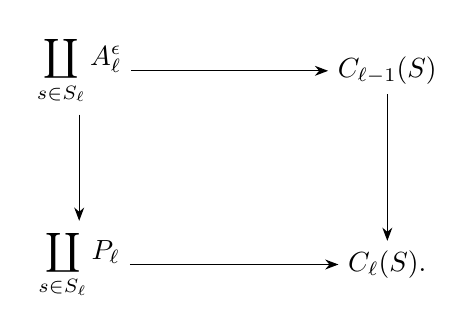
\begin{tikzpicture}[baseline=(current bounding box.center),
                   node distance=1.35cm and 2.5cm,>=Stealth]
\node (a) {\(\displaystyle\coprod_{s\in S_\ell} A_\ell^\epsilon\)};
\node (b) [right=of a] {\(C_{\ell-1}(S)\)};
\node (c) [below=of a] {\(\displaystyle\coprod_{s\in S_\ell} P_\ell\)};
\node (d) at (b |- c) {\(C_\ell(S)\).};
\draw[->] (a) -- (b);
\draw[->] (a) -- (c);
\draw[->] (b) -- (d);
\draw[->] (c) -- (d);
\end{tikzpicture}
\end{equation}
Here \(S_\ell\) is the set of actual \(\ell\)-cells of the
globular set \(S\).  If \(S\) is a pasting scheme, then
\begin{equation}\label{eq:cylinder-skeletal-ends}
 C_n(S)=H_\epsilon(S),\qquad
 C_{j-1}(d_j)=A_j^\epsilon\quad(j>n),\qquad
 C_{\dim(S)}(S)=P(S).
\end{equation}
The first identity uses the whisker orientation for which the retained
copy of \(S\) is endpoint \(\epsilon\).
\end{lemma}

\begin{proof}
The ordinary skeleton \(\sk_\ell S\) is obtained from
\(\sk_{\ell-1}S\) by attaching one globe along its boundary for
each \(s\in S_\ell\).  Both \(F\) and the construction
\(P(-)\) in Equation~\eqref{eq:cylinder-realization} preserve these
colimits.  More explicitly, a map \(C_\ell(S)\to T\) consists of
a map \(F(S)\to T\) and maps from its cylinder objects through
level \(\ell\), compatible on faces and on endpoint
\(\epsilon\).  After specifying the same data through level
\(\ell-1\), extending them at a particular cell \(s\) amounts
to choosing a map \(P_\ell\to T\) with its values already
prescribed on \(P(\partial d_\ell)\) and on the retained
endpoint \(D_\ell\).  Those prescribed values form precisely a
map \(A_\ell^\epsilon\to T\).  This is the universal property
of Equation~\eqref{eq:cylinder-skeletal-pushout}.

In particular, faces shared by two cells use the same map from the
previous skeleton.  No additional copy of a shared face is introduced.
The argument concerns colimits of the specified cylinder objects, so it
also applies when an earlier upper completion has attached cells of
dimension less than its cylinder index.

Through dimension \(n-1\), all the cylinders are stationary.  At
dimension \(n\), each cell acquires one duplicate and one joining
cell; the original higher cells retain their original boundaries.
This proves \(C_n(S)=H_\epsilon(S)\), including the case
\(\dim(S)<n\), in which there are no whiskers.  The other two
identities follow from \(\sk_{j-1}d_j=\partial d_j\) and
\(\sk_{\dim(S)}S=S\), respectively.
\end{proof}

\begin{proposition}\label{prop:cylinder-contractibility}
Every \(P_j\) is contractible.  For \(n<j\le q\), both
one-sided domains \(A_j^\epsilon\) are contractible, and
\(A_j^\epsilon\to P_j\) is an upper cellular weak equivalence.
For every pasting scheme \(S\) of height at most \(q\), the model
\(P(S)\) is cellular and contractible.
\end{proposition}

\begin{proof}
The objects \(P_j\) for \(j\le n\) are free globes and are
contractible by Proposition~\ref{prop:shape-contractible}.  Proceed
by induction on \(j>n\), handling both endpoints.  By
Lemma~\ref{lem:cylinder-skeletal-gluing}, \(A_j^\epsilon\) is
obtained from \(H_\epsilon(d_j)\) by pushing out the maps
\(A_\ell^\epsilon\to P_\ell\) on the boundary cells of
dimensions \(n<\ell<j\), in increasing order of \(\ell\).
At each dimension, attach its finitely many cells one at a time.
The resulting iterated pushout is the coproduct pushout of
Lemma~\ref{lem:cylinder-skeletal-gluing}, by its universal property.
The starting object is cellular and contractible by
Proposition~\ref{prop:whiskered-shape}.  Each map used in this
filtration is already an upper cellular weak equivalence by the
induction on \(j\).  Lemma~\ref{lem:upper-cell} therefore makes
every one of its pushouts a weak equivalence.  All intermediate objects
are cellular, so the lemma applies at every stage.  It follows that
\(A_j^\epsilon\) is contractible.  When \(j=n+1\), this
filtration has no intervening stages:
\(A_{n+1}^\epsilon=H_\epsilon(d_{n+1})\).

The upper cellular map \(A_j^\epsilon\to P_j\) preserves all
cells through dimension \(n\), by Lemma~\ref{lem:high-cells}.
Thus \(P_j\) is nonempty and inherits fillers of dimensions
\(1,\ldots,n\) from \(A_j^\epsilon\).  Its map to the
terminal object lifts the upper boundary inclusions by construction,
so it has every remaining boundary filler.  Hence \(P_j\) is
contractible.  At \(n=0\), the inherited condition is simply
nonemptiness.  Both terminal maps are now weak equivalences, so
\(A_j^\epsilon\to P_j\) is a weak equivalence.  Its upper
cellularity was established in Equation~\eqref{eq:cylinder-upper-one-sided}.
This completes the induction on \(j\).

For a pasting scheme \(S\) with \(\dim(S)\ge n\), start with
\(C_n(S)=H_\epsilon(S)\) and use the same filtration through
all dimensions \(n<\ell\le\dim(S)\).  It ends at \(P(S)\).
Every step is again a cellular weak equivalence by
Lemma~\ref{lem:upper-cell}; its cellular, contractible starting object
therefore gives the assertion.  If \(\dim(S)<n\), then
\(P(S)=F(S)\), so Proposition~\ref{prop:shape-contractible}
applies directly.
\end{proof}

\subsection{Interpreting every operation of the coherator}

Contractibility of \(P(S)\) is the output needed from the geometric
construction.  It will let us extend each operation from its already
prescribed boundary and endpoints.  Making that extension once on the
representing objects will ensure naturality in the model.

For \(Y\in\mathcal A_q\), form the globular set with cells
\begin{equation}\label{eq:partial-path-cells}
           (\mathcal P Y)_j=\Hom_{\mathcal A_q}(P_j,Y),
                     \qquad 0\le j\le q,
\end{equation}
and complete it above dimension \(q\) by unique fillers of all
boundaries.  The coglobular identities give its globular identities.
Precomposition with \(e_\epsilon\) gives globular maps
\(p_\epsilon:\mathcal P Y\to Y\) through dimension \(q\),
which extend uniquely above it.  Equation~\eqref{eq:cylinder-realization}
gives the natural representation
\begin{equation}\label{eq:partial-path-tuples}
 \{\text{globular maps }S\to\mathcal P Y\}
       \cong\Hom_{\mathcal A_q}(P(S),Y)
             \qquad(\dim(S)\le q).
\end{equation}

\begin{proposition}\label{prop:partial-path}
The construction in Equation~\eqref{eq:partial-path-cells} admits
interpretations of every operation of \(\mathcal C\), making
\(\mathcal P:\mathcal A_q\to\mathcal A_q\) a functor and
both \(p_\epsilon\) natural model morphisms.  They lift all
boundary inclusions \(I_j\).  Their joint map
\[
              (p_0,p_1):\mathcal P Y\longrightarrow Y\times Y
\]
lifts \(J_n\).
\end{proposition}

\begin{proof}[Construction of the algebraic interpretation]
Interpret the generators in the \emph{original free construction order}
of \(\mathcal C\).  At each stage, the globular set
\(\mathcal P Y\) already interprets the entire preceding theory,
naturally in the full model \(Y\), and both endpoints preserve that
preceding theory.  This holds initially for the globular structure.

Consider a new generating filler \(\theta\), of output dimension
\(j>0\), on a pasting-scheme arity \(S\).  If \(j>q\),
evaluate its already interpreted boundary and take its unique filler
in \(\mathcal P Y\).  The endpoint equations follow from the
boundary equations and unique fillers in \(Y\).  This is natural
in \(Y\).

Suppose \(j\le q\).  The generator condition gives
\(\dim(S)\le j\), so Equation~\eqref{eq:partial-path-tuples}
applies.  If \(j<n\), the entire tuple lies in stationary
dimensions: \(P(S)=F(S)\) and \(P_j=D_j\).  Use the original
operation of \(Y\).  Its prescribed boundary follows from the
preceding endpoint compatibility, since the endpoint maps are identical
isomorphisms on all the cell sets involved.

It remains to handle \(n\le j\le q\).  View the given operation,
in the fixed category of full models, as a map
\[
                         \theta:D_j\longrightarrow F(S).
\]
This map exists independently of the interpretation being constructed
on \(\mathcal P Y\).  Its required endpoint values are the two
existing maps
\begin{equation}\label{eq:partial-path-endpoint-prescription}
             e_\epsilon(S)\theta:D_j\longrightarrow P(S).
\end{equation}
The two face operations of \(\theta\) belong to the preceding
theory.  Evaluating either one on an \(S\)-tuple gives, naturally
in \(Y\), a function
\[
 \Hom_{\mathcal A_q}(P(S),Y)
       \longrightarrow\Hom_{\mathcal A_q}(P_{j-1},Y).
\]
By Yoneda, these functions are represented by maps
\(P_{j-1}\to P(S)\).  Their parallelism is an equation in the
preceding theory, so they agree on all their common faces and give
\[
                 b_\theta:P(\partial d_j)\longrightarrow P(S).
\]
The previous endpoint compatibility says exactly that
\begin{equation}\label{eq:partial-path-boundary-compatibility}
 b_\theta e_\epsilon(\partial d_j)
       =e_\epsilon(S)(\theta|_{\partial D_j}).
\end{equation}
Consequently \(b_\theta\) and the two maps in
Equation~\eqref{eq:partial-path-endpoint-prescription} glue to a map
\begin{equation}\label{eq:partial-path-two-sided-prescription}
                         A_j^{01}\longrightarrow P(S).
\end{equation}

The map \(A_j^{01}\to P_j\) is cellular for
\(n\le j\le q\), and \(P(S)\) is contractible by
Proposition~\ref{prop:cylinder-contractibility}.  Its terminal map
therefore lifts every boundary inclusion, and hence every cellular map.
It extends Equation~\eqref{eq:partial-path-two-sided-prescription} to
a map \(P_j\to P(S)\).  Precomposition with this chosen map is
the required operation on \(\mathcal P Y\).  Its boundary and
endpoint equations hold by construction.

In this step a face operation can be a composite of output dimension
\(j-1\) whose arity \(S\) has height \(j\).  Its evaluation
and Yoneda representation use the whole preceding theory.  Preservation
of its generators makes the endpoints preserve all their composites
and substitutions as well.  The inequality \(\dim(S)\le j\)
was used for the new generator; no smaller arity bound on its composite
faces is needed.

Make the representing choices once, independently of \(Y\).
Postcomposition by a map \(Y\to Z\) then preserves every
chosen operation.  At limit stages of the free theory, the compatible
interpretations give the interpretation of its union.  Freeness now
provides a model of the full \(\mathcal C\), natural in \(Y\),
and both endpoints are full model morphisms.  The construction leaves
the chosen globular set unchanged; it is therefore still
\(q\)-coskeletal.
\end{proof}

\begin{proof}[Lifting for an individual endpoint]
For \(j\le q\), an \(I_j\)-lifting problem against
\(p_\epsilon\) specifies a boundary cylinder and one endpoint
disk with matching endpoint boundary.  By
Equation~\eqref{eq:cylinder-one-sided}, it is a map
\(A_j^\epsilon\to Y\), and a solution is an extension to
\(P_j\to Y\).

For \(j<n\), the map \(A_j^\epsilon\to P_j\) is the
identity.  For \(j=n\), it is one face inclusion
\(D_n\to D_{n+1}\), which has a retraction given by a unit
operation.  For \(j>n\), it is an upper cellular weak equivalence
by Proposition~\ref{prop:cylinder-contractibility}, and has a
retraction by Lemma~\ref{lem:upper-cell}.  Precomposing with these
retractions gives the desired extensions into every \(Y\).
For \(j>q\), the map \(I_j\) is an isomorphism in
\(\mathcal A_q\).  Thus both endpoints lift all \(I_j\),
and belong to \(\mathcal W\) by Lemma~\ref{lem:lifting-test}.
\end{proof}

\begin{proof}[Lifting for the joint endpoint]
A lifting problem against \(J_n\) consists of a map
\(h:P_n\to Y\) and two maps \(a_0,a_1:D_{n+1}\to Y\)
whose source faces are the two endpoints of \(h\).  Its representing
object is
\begin{equation}\label{eq:partial-path-tree-domain}
 B=P_n\amalg_{D_n\amalg D_n}(D_{n+1}\amalg D_{n+1}),
\end{equation}
where the attaching maps use the two endpoints of \(P_n\) and
the source of each new disk.  Since \(P_n=D_{n+1}\), its
presentation in the depth-\(n\) slot has four \(n\)-cells and
three \((n+1)\)-cells:
\[
 h:x_0\longrightarrow x_1,\qquad
 a_0:x_0\longrightarrow y_0,\qquad
 a_1:x_1\longrightarrow y_1.
\]
For \(n>0\), the four \(n\)-cells have their common lower
globular boundary.  For \(n=0\), they are four ordinary vertices.
The underlying graph is the tree \(y_0-x_0-x_1-y_1\).
Thus \(B\) is cellular and contractible by
Proposition~\ref{prop:tree-contractible}.

\begin{fixedfigure}
\centering
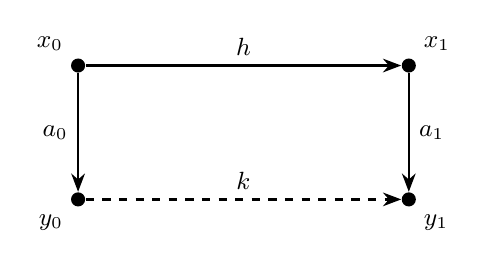
\begin{tikzpicture}[>=Stealth,
    vertex/.style={circle,fill=black,inner sep=1.8pt},
    every node/.style={font=\small}]
\node[vertex,label=above left:\(x_0\)] (x0) at (0,1.7) {};
\node[vertex,label=above right:\(x_1\)] (x1) at (4.2,1.7) {};
\node[vertex,label=below left:\(y_0\)] (y0) at (0,0) {};
\node[vertex,label=below right:\(y_1\)] (y1) at (4.2,0) {};
\draw[->,thick] (x0) -- node[above] {\(h\)} (x1);
\draw[->,thick] (x0) -- node[left] {\(a_0\)} (y0);
\draw[->,thick] (x1) -- node[right] {\(a_1\)} (y1);
\draw[->,thick,dashed] (y0) -- node[above] {\(k\)} (y1);
\end{tikzpicture}
\caption{The solid arrows form the tree representing the joint-endpoint
lifting data \(B\).  Vertices denote \(n\)-cells and arrows denote
\((n+1)\)-cells; all vertices have the same lower boundary when \(n>0\).
Adjoining the dashed comparison \(k\) is one upper boundary attachment
\(I_{n+1}\), giving \(A_{n+1}^{01}\).  The square depicts boundary
data; its higher filling cells belong to the remaining upper completion,
which gives \(P_{n+1}\).}
\label{fig:joint-endpoints}
\end{fixedfigure}


The cylinder on the source \(n\)-face is already \(P_n\).
Attach the missing comparison \(y_0\to y_1\), one
\((n+1)\)-cell, to supply the cylinder on the target face.  Together
with the two endpoint disks this is exactly
\(A_{n+1}^{01}\).  Hence the natural map to \(P_{n+1}\)
factors as
\[
                 B\longrightarrow A_{n+1}^{01}
                        \longrightarrow P_{n+1},
\]
where the first map is one \(I_{n+1}\)-attachment and the second
is the chosen upper completion.  It is an upper cellular map between
cellular contractible objects, so it is a weak equivalence and splits
by Lemma~\ref{lem:upper-cell}.  A retraction
\(P_{n+1}\to B\), followed by the prescribed map \(B\to Y\),
solves the lifting problem.  This also applies when \(q=n+1\):
the missing comparison is a legitimate \(I_q\)-attachment, and
all subsequent required fillers are provided by the same construction.
This completes the proof of Proposition~\ref{prop:partial-path}.
\end{proof}

\subsection{An arbitrary attaching cell}

\begin{proof}[Completion of the descending induction]
Let \(X\) be cellular in \(\mathcal A_q\), let
\(a:D_n\to X\) be arbitrary, and form the algebraic pushout
\[
              Y=X\amalg_{D_n}D_{n+1},\qquad i:X\longrightarrow Y.
\]
The unit on \(a\) gives the elementary retraction
\(r:Y\to X\), with \(ri=\id_X\).  Because
\(p_0:\mathcal P X\to X\) lifts every boundary inclusion and
\(X\) is cellular, there is a map \(h:X\to\mathcal P X\)
with \(p_0h=\id_X\).  Set
\[
                  u=p_1h:X\longrightarrow X,
             \qquad \bar u=ur:Y\longrightarrow X.
\]
Both endpoints are weak equivalences; thus two-out-of-three first gives
\(h\in\mathcal W\) and then \(u\in\mathcal W\).
Also \(\bar u i=u\).

Consider the square
\begin{equation}\label{eq:partial-path-final-square}
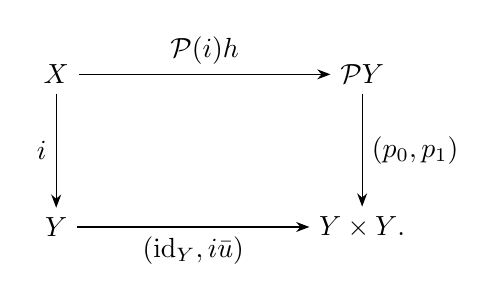
\begin{tikzpicture}[baseline=(current bounding box.center),
                   node distance=1.45cm and 3.2cm,>=Stealth]
\node (a) {\(X\)};
\node (b) [right=of a] {\(\mathcal P Y\)};
\node (c) [below=of a] {\(Y\)};
\node (d) at (b |- c) {\(Y\times Y\).};
\draw[->] (a) -- node[above] {\(\mathcal P(i)h\)} (b);
\draw[->] (a) -- node[left] {\(i\)} (c);
\draw[->] (b) -- node[right] {\((p_0,p_1)\)} (d);
\draw[->] (c) -- node[below] {\((\id_Y,i\bar u)\)} (d);
\end{tikzpicture}
\end{equation}
Naturality and \(\bar u i=u\) give its commutativity explicitly:
\[
 (p_0,p_1)\mathcal P(i)h=(i,iu)
                         =(\id_Y,i\bar u)i.
\]
The right-hand map lifts \(J_n\) by
Proposition~\ref{prop:partial-path}, so it lifts its pushout \(i\).
Indeed, restrict the top map along the given \(a:D_n\to X\),
and restrict the bottom map along the new disk
\(D_{n+1}\to Y\).  Solve this \(J_n\)-square; its solution
agrees with the original top map on \(D_n\), and the actual pushout
universal property glues the two maps.  This produces
\(f:Y\to\mathcal P Y\) with
\[
                  p_0f=\id_Y,\qquad p_1f=i\bar u.
\]
This use of the pushout requires no condition on the selected cell
\(a\) beyond being a model morphism from \(D_n\).
Two-out-of-three again gives
\[
                         v:=i\bar u\in\mathcal W.
\]

Finally, \(iu:X\to Y\) is a retract of \(v=iur:Y\to Y\)
in the arrow category.  The maps of arrows in the two directions have
domain maps \(i\) and \(r\), respectively, and codomain map
\(\id_Y\) in both cases.  The identities
\[
                vi=iu,\qquad (iu)r=v,\qquad ri=\id_X
\]
verify the two commuting squares and their identity composite.
Retract closure gives \(iu\in\mathcal W\), and two-out-of-three
with \(u\in\mathcal W\) gives \(i\in\mathcal W\).
Every map in this argument is a morphism of the full algebraic models;
the conclusion therefore includes all freely generated composites and
coherence cells of the pushout, for the arbitrary attaching cell \(a\).

This proves the induction step at \(n\).  Together with the top
case established in the preceding section, descending induction proves
the elementary expansion assertion for every index at this fixed
cutoff \(q\).
\end{proof}

\begin{proof}[Proof of Theorem~\ref{thm:main}]
Return to the original category \(\mathcal A\), and write
\(i:X\to Y\) for the pushout in the theorem.  Fix an instance of
the exact-boundary test in dimension \(k\).  Choose
\(q\ge\max\{n+1,k+1\}\).  By Lemma~\ref{lem:cutoff}, the
reflector \(R_q\) preserves the cellular presentation of \(X\)
and the actual pushout defining \(Y\).  The fixed-cutoff theorem
therefore applies to \(R_q(i)\).

The reflector preserves all cells through dimension \(q\), with
their face maps.  Consequently the given boundary and target disk are
unchanged by reflection.  The source disk and its \((k+1)\)-cell
homotopy supplied by the fixed-cutoff theorem are also in unchanged
dimensions.  They are therefore a source disk with the original exact
boundary and an actual homotopy in \(Y\) before reflection.
Proposition~\ref{prop:weak-test} proves that \(i\) is a weak
equivalence.  This holds for every \(k\), every \(n\ge0\),
every cellular \(X\), and the arbitrary fixed coherator
\(\mathcal C\), as required.
\end{proof}

\section{Semi-model structure and the homotopy hypothesis}
\label{sec:consequences}

We now apply the expansion theorem to the original category
\(\mathcal A=\Mod(\mathcal C)\), without a coskeletal cutoff.
The first consequence is the canonical structure of
\cite[Theorem~5.3.5]{Henry2016}.  We give its transfer argument explicitly
to distinguish cellular objects from their cofibrant retracts.

\subsection{The canonical semi-model structure}

Recall
\[
 I=\{I_j:\partial D_j\longrightarrow D_j\mid j\ge0\},
 \qquad
 J=\{J_j:D_j\longrightarrow D_{j+1}\mid j\ge0\}.
\]
For a set of maps \(K\), write \(K\text{-}\mathrm{cof}\)
for the maps with the left lifting property
against \(K\text{-}\mathrm{inj}\).

We use the left semi-model convention in which
cofibration--trivial-fibration factorization and lifting hold for all maps.
Trivial-cofibration--fibration factorization and lifting are required for maps
with cofibrant domain.  The proof below verifies these restrictions
explicitly.

\begin{corollary}\label{cor:semimodel}
For every Grothendieck coherator \(\mathcal C\), the category
\(\mathcal A\) admits a cofibrantly generated left semi-model structure
with
\[
 \begin{aligned}
  \text{weak equivalences}&=\mathcal W,\\
  \text{cofibrations}&=I\text{-}\mathrm{cof},\\
  \text{fibrations}&=J\text{-}\mathrm{inj},\\
  \text{trivial fibrations}&=I\text{-}\mathrm{inj}.
 \end{aligned}
\]
Here \(\mathcal W\) is the class defined by components and based
homotopy groups.  Cofibrant objects are exactly retracts of cellular
objects, and every object is fibrant.
\end{corollary}

\begin{proof}
Each \(J_j\) is a composite of two boundary attachments: an
\(I_j\)-attachment adds the parallel \(j\)-cell, and an
\(I_{j+1}\)-attachment adds the cell joining the two.  Consequently
\(J\subset I\text{-}\mathrm{cof}\).  The lifting calculation of
Lemma~\ref{lem:lifting-test} gives
\begin{equation}\label{eq:consequences-trivial-fibrations}
 I\text{-}\mathrm{inj}
   =\mathcal W\cap J\text{-}\mathrm{inj}.
\end{equation}
Indeed an \(I\)-injective map satisfies the exact-boundary test and
lifts \(J\); conversely, for a weak equivalence lifting \(J\), first
lift a disk up to one higher homotopy and then lift that homotopy to
correct the disk exactly.

The small object argument for \(I\) supplies a weak factorization
system
\[
 \bigl(I\text{-}\mathrm{cof},\ I\text{-}\mathrm{inj}\bigr)
\]
on all maps.  In particular, factoring \(\varnothing\to X\) shows
that every cofibrant \(X\) is a retract of a cellular object: the
cofibrancy of \(X\) provides a section of the resulting trivial
fibration onto \(X\).  The converse follows from closure of the left
lifting class under retracts.

Theorem~\ref{thm:main} extends from cellular starts to cofibrant starts.
To see this explicitly, choose a retract diagram
\(X\xrightarrow{u}Z\xrightarrow{v}X\), with \(vu=\id_X\) and
\(Z\) cellular.  Given \(a:D_j\to X\), form the two expansions
\[
 X^+=X\amalg_{D_j,a}D_{j+1},
 \qquad
 Z^+=Z\amalg_{D_j,ua}D_{j+1}.
\]
The maps \(u,v\), together with the identity on the new
\(D_{j+1}\), induce maps \(X^+\to Z^+\to X^+\) whose composite
is the identity.  Thus \(X\to X^+\) is a retract of \(Z\to Z^+\)
in the arrow category and belongs to \(\mathcal W\).

Every relative \(J\)-cell map with cofibrant domain is therefore a
weak equivalence.  Cofibrancy is preserved at each stage because every
\(J_j\) is an \(I\)-cofibration.  At successor stages use the
preceding paragraph, and at limit stages use the filtered-colimit
closure of \(\mathcal W\) from Lemma~\ref{lem:weak-closure}.
A set of simultaneous attachments can equally be attached in any
well-order, so this also covers the coproducts used by the small object
argument.  The small object argument for \(J\) consequently factors
every map with cofibrant domain as
\[
 X\xrightarrow{j}Z\xrightarrow{p}Y,
 \qquad
 j\in I\text{-}\mathrm{cof}\cap\mathcal W,
 \quad p\in J\text{-}\mathrm{inj}.
\]
As a relative \(J\)-cell map, \(j\) has the left lifting property
against every fibration.

Conversely, let \(i:X\to Y\) be an \(I\)-cofibration and a weak
equivalence, with \(X\) cofibrant.  Apply this factorization to \(i\),
writing \(i=pj\).  Two-out-of-three puts \(p\) in \(\mathcal W\),
so Equation~\eqref{eq:consequences-trivial-fibrations} makes \(p\)
\(I\)-injective.  A lift of \(i\) against \(p\) exhibits \(i\)
as a retract of \(j\).  Hence every trivial cofibration with
cofibrant domain lifts against every fibration.

These are precisely the required factorizations and lifting axioms:
cofibration--trivial-fibration factorization and lifting hold without
restriction, while trivial-cofibration--fibration factorization and
lifting are required for cofibrant domains.  Completeness and
cocompleteness follow from the algebraic description of \(\mathcal A\);
the retract and two-out-of-three axioms were proved in
Lemma~\ref{lem:weak-closure}.  Finally, the unit of a \(j\)-cell
extends it along \(J_j\).  Thus every map \(X\to 1\) is
\(J\)-injective, and every object is fibrant.
\end{proof}

\subsection{The comparison with spaces}

We use the cylinder-category comparison established in
\cite[Sections~5.1 and~5.3]{Henry2016}.  The relevant implication is
all-dimensional and has exactly the expansion assertion as its
additional hypothesis.  We spell out its application to the fixed
coherator.

The comparison first packages finite cellular models and their
cylinders into a small category.  Its completion recovers all models
of the same coherator.  Henry's recognition theorem then identifies
that completion with spaces up to Quillen equivalence.  The proof
below records the hypotheses at each of these three interfaces.

A cylinder category has cofibrations and weak equivalences satisfying
\cite[Definition~2.1.1]{Henry2016}; in particular, it has cofibration
pushouts, its weak equivalences satisfy two-out-of-six, every object
has a cylinder, and every trivial cofibration retracts.  Its completion
is the full category of set-valued presheaves taking the initial object
to a singleton and cofibration pushouts to pullbacks
\cite[Definition~2.4.1]{Henry2016}.

Here \(\Spaces\) denotes the usual model category of topological spaces,
with weak homotopy equivalences.

\begin{corollary}\label{cor:homotopy-hypothesis}
For every Grothendieck coherator \(\mathcal C\), the canonical
semi-model category \(\Mod(\mathcal C)\) is Quillen equivalent to
spaces.  More precisely, there is a geometric-realization/fundamental-
infinity-groupoid adjunction
\[
 |-|:\Mod(\mathcal C)\ \rightleftarrows\ \Spaces:\Pi_\infty
\]
which is a Quillen equivalence.  In particular,
\[
 \Mod(\mathcal C)[\mathcal W^{-1}]
       \simeq \operatorname{Ho}(\Spaces).
\]
Thus the Grothendieck homotopy hypothesis holds for these groupoids.
\end{corollary}

\begin{proof}
Let \(\mathcal A_{\mathrm{fin}}\) be a small skeleton of the full
subcategory of finitely cellular \(\mathcal C\)-groupoids, with finite boundary-cell
extensions as cofibrations and the restriction of \(\mathcal W\)
as weak equivalences.  Henry's comparison uses the following three
facts.

First, under the expansion assertion, \(\mathcal A_{\mathrm{fin}}\)
is a cylinder category
\cite[Proposition~5.3.6]{Henry2016}.  The finite nature of its
cylinders is explicit: a relative cylinder for the generating
cofibration \(\partial D_j\to D_j\) is
\[
 D_j\amalg_{\partial D_j}D_j
       \longrightarrow D_{j+1}\longrightarrow D_j.
\]
The first map is \(I_{j+1}\), and the source endpoint is \(J_j\);
the last map is induced by a unit.  The source endpoint is a weak
equivalence by Theorem~\ref{thm:main}, and hence so is the last map.
Finite relative cylinders are obtained by the finite cell induction
of that proposition.  Trivial cofibrations in this category have
retractions by Corollary~\ref{cor:semimodel}, since their domains are
cofibrant and all objects are fibrant.

Second, the free construction of the original coherator identifies
the completion of \(\mathcal A_{\mathrm{fin}}\) with
\(\Mod(\mathcal C)\), equipped with precisely the structure in
Corollary~\ref{cor:semimodel}
\cite[Proposition~5.3.7]{Henry2016}.  In this construction one begins
with finite globular sets and adjoins the operations in the given
free order of \(\mathcal C\).  Thus the identification retains the
chosen theory and its actual algebraic models.  The generating
cofibrations in the completion are the \(I_j\), and its generating
trivial cofibrations are the relative-cylinder endpoints \(J_j\).

Third, the marked object \(D_0\) makes
\(\mathcal A_{\mathrm{fin}}\) a cylinder coherator
\cite[Corollary~5.3.12]{Henry2016}.  In Henry's terminology this
means that the map from the free pre-cylinder category \(F_*\) on one object,
selecting \(D_0\), is a trivial cofibration and that the target is a
cylinder category \cite[Definition~5.1.1]{Henry2016}.
The hypotheses used in this implication are the
free cellular construction of \(\mathcal C\), the expansion
assertion, and the homotopical terminality of \(D_0\).  The first is
part of Definition~\ref{def:coherator}, the second is
Theorem~\ref{thm:main}, and the third follows here also from
Proposition~\ref{prop:shape-contractible}: the map \(D_0\to1\)
is \(I\)-injective by the boundary-filling characterization of
contractibility.  Every map \(A\to D_0\) therefore extends across
every finite cellular cofibration \(A\to B\); this gives
homotopical terminality inside \(\mathcal A_{\mathrm{fin}}\).
More explicitly, the projection
\(p:\mathcal A_{\mathrm{fin}}^{D_0}\to\mathcal A_{\mathrm{fin}}\)
in Henry's construction is an acyclic fibration by
\cite[Proposition~4.4.4]{Henry2016}.\footnote{The phrase
``trivial cofibration'' for this projection in the proof of
\cite[Lemma~5.3.11]{Henry2016} is a typographical error;
Proposition~4.4.4 gives an acyclic fibration.}
The relative cofibrancy of \(F_*\to\mathcal A_{\mathrm{fin}}\)
from \cite[Proposition~5.3.7]{Henry2016} therefore gives a section
of \(p\) sending the marked \(D_0\) to its cylinder \((D_0,D_1)\).
The lifting argument of \cite[Lemma~5.3.9]{Henry2016} then gives
the asserted cylinder-coherator property, as in
\cite[Lemma~5.3.11 and Corollary~5.3.12]{Henry2016}.

Henry's Theorem~5.1.2(5) now gives a fundamental-infinity-groupoid
right Quillen equivalence from spaces to this completion, with
geometric realization as its left adjoint.  By the second step the
completion is the original \(\Mod(\mathcal C)\) with its canonical
weak equivalences.  This proves the displayed statements and is the
implication summarized in \cite[Corollary~5.3.13]{Henry2016}.
\end{proof}

\bibliographystyle{plain}
\bibliography{references}
\end{document}
